\documentclass[titlepage]{jsreport}

\usepackage[dvipdfmx]{graphicx}
\usepackage[dvipdfmx]{color}
\usepackage{listings, jlisting}
\usepackage{cite}
\usepackage{url}
\usepackage{subcaption}

% ソースコードを挿入するための設定
\lstset{
language={Python},
basicstyle={\ttfamily\small},
backgroundcolor={\color[gray]{.95}},
keywordstyle={\color[rgb]{0.0,0.0,0.8}},
commentstyle={\color[rgb]{0.5,0.5,0.5}},
stringstyle={\color[rgb]{0.0,0.5,0.5}},
frame=single,
numbers=left,
numberstyle={\ttfamily\small},
breaklines=true,
breakindent = 10pt,
tabsize=2,
captionpos=t
}

\title{卒業論文のタイトル}
\author{慶應義塾大学理工学部物理情報工学科\\
指導教員 渡辺宙志\\
学籍番号 62116135\\
深瀬遥斗}
\date{2025年3月}

\begin{document}
\pagenumbering{roman}
\maketitle
\setcounter{tocdepth}{2}
\tableofcontents

\chapter{はじめに} \label{chap:introduction}
\pagenumbering{arabic}

「はじめに」もしくは「緒言」では、研究背景、目的、そして論文の構成を書く。第一章の前に目次をつける場合、目次のページ番号はi, ii,とローマ数字にして、本文からアラビア数字にするのが一般的だ。それを実現するため、\verb|\begin{document}|の直後にページ番号をローマ数字にするコマンド\verb|\pagenumbering{roman}|が、最初の\verb|\chapter|の後にアラビア数字にするコマンド\verb|\pagenumbering{arabic}|が挿入されている。

\section{研究の背景}

研究の背景は「なぜこの研究をしなければならないか」を、「大きい理由から小さい理由」へ書いていく。「大きい理由」は、「エネルギー問題」「安全」「便利」といった、「多くの人がほぼ納得するような理由」を挙げる。次に、その「大きな理由」を実現するために、これまでどのような試みがなされてきたかを説明する。これまでに読んだ論文のイントロダクションを参考に、必要な文献を引用しながら説得力のある文章を書くこと。

\section{研究の目的}

研究の背景を受けて、この研究分野は重要であるが、なんらかの不満点があることを述べる。その不満点は解決すべき問題であることを文献を引用しながら読者に納得させる。本研究の目的は、その不満点を解消することであることを述べ、その方法について簡単に述べる。

\section{本論文の構成}

論文の構成を説明する。まず本研究の目的を一行で書いてから、各章に何が書いてあるかを説明する。以下は例である。

\begin{quotation}
    本研究では、では、分野Aにおける手法Xの精度改善を行う。以下に本論文の構成を示す。第\ref{chap:introduction}章では、分野Aにおける手法の概観を紹介し、手法Xが広く用いられていることを示した。第\ref{chap:method}章では、本研究で用いる手法X、及びその改善手法であるX'について説明する。第\ref{chap:results}章では、本研究で提案した手法X'と、もととなった手法Xとの精度の比較を行う。第\ref{chap:summary}章では本研究で得られた知見を総括し、結論と今後の展望について述べる。
\end{quotation}

\chapter{原理} \label{chap:principle}

\section{売買価格の決定方法}
\subsection{売買契約の優先順位}
東証の取引所市場において売買立会による取引は,価格優先の原則と時間優先の原則に従い,競争売買によって行われる\cite{shokengaimuin}.
価格優先の原則とは,売呼値は低い値段の注文を,買呼値は高い値段の注文を優先して成立させるという取引上のルールである.
一方で時間優先の原則では,注文した時間の早かった注文が優先して成立されるが,時間優先の原則より価格優先の原則を先に適用させるため,時間優先の原則は同一値段の呼値に対してのみ適用される.
また,時間や価格に関係なく成行呼値は指値による呼値より優先される.

\subsection{板寄せとザラ場方式}
売買価格の決定方法には,始値や終値を定める場合に用いられる板寄せと,始値決定後の値段の決定に用いられるザラ場方式がある\cite{shokengaimuin}.

板寄せは図\ref{fig:itayose}で示すように,売注文も買い注文も成行注文を優先して対当させる.
次に残りの成行注文と,指値注文を価格優先の原則に従って対当させていく.
最後に同じ呼値同士を時間優先の原則に従って対当させることで,図\ref{fig:continuous}のようになり,始値は最後に対当させた価格である100となる.

\begin{figure}[htbp]
    \centering
    \begin{subfigure}[b]{0.49\linewidth}
        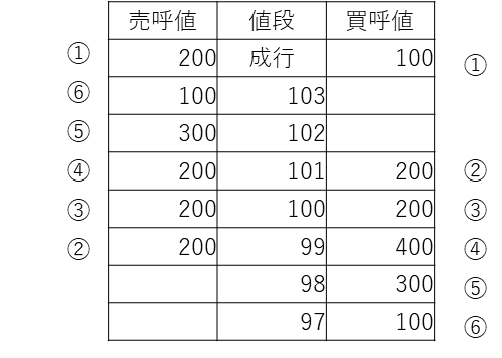
\includegraphics[width=\linewidth]{fig/itayose.pdf}
        \caption{}
        \label{fig:itayose}
    \end{subfigure}
    \hfill
    \begin{subfigure}[b]{0.335\linewidth}
        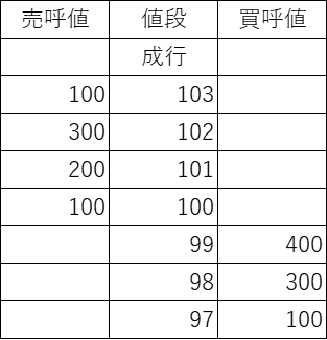
\includegraphics[width=\linewidth]{fig/continuous.pdf}
        \caption{}
        \label{fig:continuous}
    \end{subfigure}
    \caption{始値直前の板の状況(a),始値直後の板の状況(b)}
    \label{fig:opening}
\end{figure}







\section{手法} \label{chap:method}










\section{引用の仕方}

\subsection{論文や書籍の引用}

原則として科学技術論文では、引用のない文章は「著者のオリジナル」であるとみなされる。LAMMPSなどのツールを使えばその関連論文を、手法の説明をするならその手法を提案した論文を引用しなければならない。

引用するのは、原則として書籍か査読論文とし、ウェブサイトの引用はさけること。特に何かの説明の参照先としてWikipediaやSlideShareなどを挙げないこと。機械学習の論文であればプレプリント(arXiv)を読むことも多いと思われるが、引用したくなるような論文はどこかのカンファレンスに採択されていることが多いので、そちらを引用すること。たとえ自分がWikipediaで知識を得たとしても、Wikipediaで引用されている文献にあたり、書籍なり論文なりを参考にすること。

参考文献は、原則としてBibTeXで管理すること。これにより、「本文で参照されていない文献を参考文献に入れてはならない」「本文で参照される順番に並べないとならない」などのルールが自動的に満たされる。

BibTeXでは、参考文献を「エントリ」と呼ばれる構造で管理する。エントリにはいくつか種別があるが、良く使うのは書籍(book)、論文(article)、プロシーディング(inproceedings)などであろう。例えば書籍は以下のようなエントリとする。

\begin{lstlisting}[language={[LaTeX]TeX}]
@book{okumura2020,
    author    = {奥村 晴彦 and 黒木 裕介},
    title     = {LaTeX2ε美文書作成入門},
    publisher = {技術評論社},
    year      = {2020}
}
\end{lstlisting}

これをTeXファイル中で以下のように引用する。

\begin{verbatim}
本論文の執筆にあたり、LaTeXの書き方については奥村・黒木の書籍を参考にした\cite{okumura2020}。
\end{verbatim}

これは以下のようにタイプセットされる。
\begin{quotation}
    本論文の執筆にあたり、LaTeXの書き方については奥村・黒木の書籍を参考にした\cite{okumura2020}。
\end{quotation}

\subsection{URLの引用}

GitHubのサイトなど、やむを得ずURLを引用する場合には、bibitemのmiscを使って以下のようにする。

\begin{lstlisting}[language=TeX]
@misc{github,
  howpublished = {\url{https://github.com/kaityo256/rbs}
},
\end{lstlisting}

例えば

\begin{verbatim}
この論文の参照実装はGitHubにて利用可能である\cite{github}。
\end{verbatim}
として引用すると、

\begin{quotation}
    この論文の参照実装はGitHubにて利用可能である\cite{github}。
\end{quotation}
となる。

\chapter{結果} \label{chap:results}

\section{図の入れ方}

図は、数が多くなければとりえあずfigといったディレクトリにまとめて入れておくと良いだろう。数が増えてきて管理が難しくなったら節ごとにわけるなど工夫すること。画像ファイルは原則としてPDFにすること。例えば\verb|temperature.pdf|を入れたいなら、

\begin{lstlisting}[language={[LaTeX]TeX}]
\begin{figure}[htbp]
    \centering
    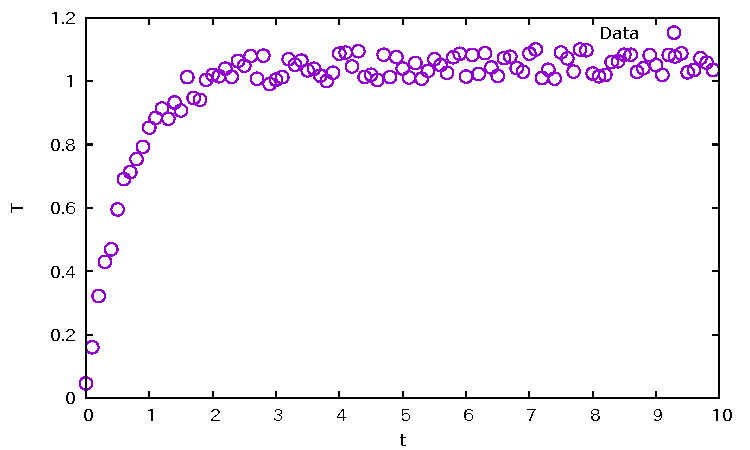
\includegraphics[width=0.49\linewidth]{fig/temperature.pdf}
    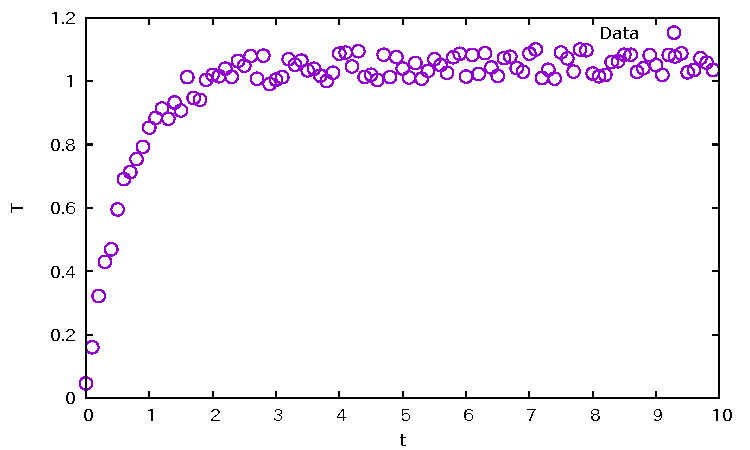
\includegraphics[width=0.49\linewidth]{fig/temperature.pdf}
    \caption{温度の時間発展。}
    \label{fig:temperature}
\end{figure}

\end{lstlisting}

とすると、以下のような図が得られる。
\begin{figure}[htbp]
    \centering
    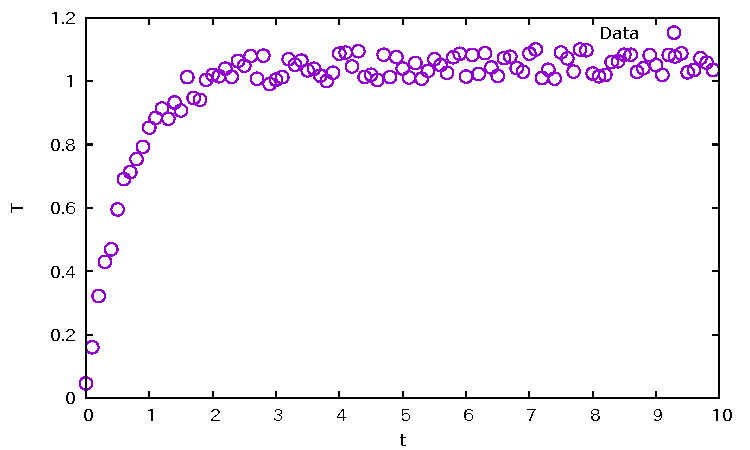
\includegraphics[width=0.49\linewidth]{fig/temperature.pdf}
    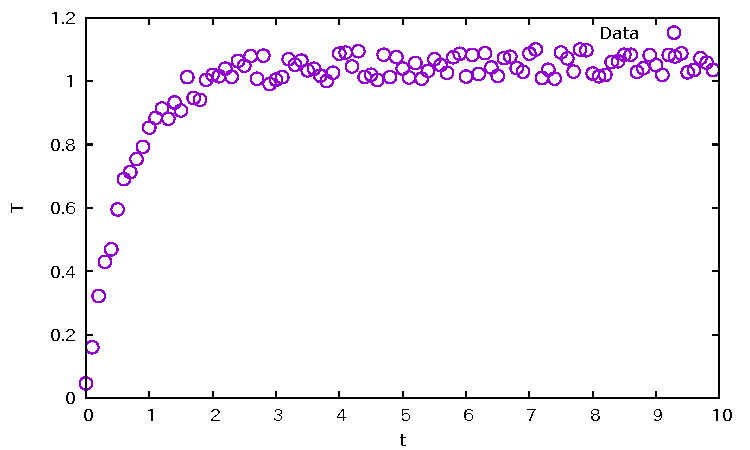
\includegraphics[width=0.49\linewidth]{fig/temperature.pdf}
    \caption{温度の時間発展。}
    \label{fig:temperature}
\end{figure}

この時、元データと、データからPDFを作るためのプロットファイルもしくはスクリプトファイルを一緒に入れておく。この時、画像ファイルとプロットファイルの名前を同じにしておくと良い。例えばgnuplotを使って\verb|temperature.pdf|という画像を作るなら、プロットファイルを\verb|temperature.plt|にしておく。すると、

\begin{lstlisting}[language=bash]
gnuplot temperature.plt
\end{lstlisting}

を実行することで\verb|temperature.pdf|ができるのでわかりやすい。

また、名前を揃えておくとmakefileとの相性が良くなる。例えば\verb|pressure.pdf|、\verb|temperature.pdf|、\verb|error.pdf|の三つのファイルが、同名のpltファイルから作成されるなら

\lstinputlisting[language=make]{fig/makefile}

といったmakefileを作っておけば、make一発で三つのファイルを作ることができるので便利だ。

もちろんPythonのMatplotlibを使っても良いが、いずれにせよ「データとスクリプトからコマンド一発で図のファイルが作成できる状況にしておく。

\chapter{考察および結論} \label{chap:summary}

考察は、「研究の背景」及び「目的」において提起した問題に正しく答えるようにする。得られた結果は満足すべきものだったか?不満があるならその理由はなにか?解決できそうなのか?また、「大きい理由」にも言及する。本研究によりどのような課題が見つかったかを書き、この分野における「研究の流れ」においてのような位置づけにあるかを説明した上で、今後、どのような発展の方向があるかについて書く。

\chapter*{謝辞}
はじめに指導教員である渡辺宙志先生にお礼申し上げます.
金融という物理情報工学科に関連のない分野にもかかわらず,研究の方向性や方法など様々な助言を送っていただいたことや,プログラミングやソフトウェアの知識に疎い私に対して丁寧に指導していただいたことなど,これらの貴重なアドバイスや指導が私の研究や成長に大いに役に立ちました.


また,研究室ミーティングや練習発表会で質問や助言を与えてくださった先輩方にも感謝しております.
特に,研究室でお会いする機会の多かった小林さんと竹内さんからは,研究への取り組み方だけでなく,自身が関心を抱く分野への取り組み方について,多くのことを学ばせていただきました.

そして,研究室の同期の皆さんにも感謝しております.
中でも伊藤君は機械の操作方法やハンズオンの内容が理解できていなかった私に対して,その都度アドバイスをくれました.
現在,私が問題なく研究を継続できているのは,伊藤君のおかげです.

最後に,これまで私を支えてくれた両親に心よりお礼申し上げます.
本研究に取り組むことができたのは,大学進学や日常生活において自由な選択肢を与え、それらを支えてくれた両親のおかげです.
ありがとうございました.

\appendix

\chapter{ソースコード}

\lstinputlisting[caption = 適当なPythonスクリプト, label = prog:sample]{src/sample.py}

\bibliographystyle{junsrt}
\bibliography{reference}

\end{document}
